\documentclass[titlepage,landscape]{seminar}
\usepackage{url}
\usepackage{graphicx}
\usepackage[pdftex]{color}
\usepackage{hyperref}
\usepackage{epstopdf}
\usepackage{slides}

\begin{document}

\myslide{\tiny
\begin{center}
\begin{tabular}{llllllll}
\hline\hline
      & Amino &       & Amino &       & Amino &       & Amino \\
Codon & Acid  & Codon & Acid  & Codon & Acid  & Codon & Acid \\
\hline
UUU   & Phe   & UCU   & Ser   & UAU   & Tyr   & UGU   & Cys \\
UUC   & Phe   & UCC   & Ser   & UAC   & Tyr   & UGC   & Cys \\
UUA   & Leu   & UCA   & Ser   & UAA   & Stop  & UGA   & Stop \\
UUG   & Leu   & UCG   & Ser   & UAG   & Stop  & UGG   & Trp \\
      &       &       &       &       &       &       & \\
CUU   & Leu   & CCU   & Pro   & CAU   & His   & CGU   & Arg \\
CUC   & Leu   & CCC   & Pro   & CAC   & His   & CGC   & Arg \\
CUA   & Leu   & CCA   & Pro   & CAA   & Gln   & CGA   & Arg \\
CUG   & Leu   & CCG   & Pro   & CAG   & Gln   & CGG   & Arg \\
      &       &       &       &       &       &       & \\
AUU   & Ile   & ACU   & Thr   & AAU   & Asn   & AGU   & Ser \\
AUC   & Ile   & ACC   & Thr   & AAC   & Asn   & AGC   & Ser \\
AUA   & Ile   & ACA   & Thr   & AAA   & Lys   & AGA   & Arg \\
AUG   & Met   & ACG   & Thr   & AAG   & Lys   & AGG   & Arg \\
      &       &       &       &       &       &       & \\
GUU   & Val   & GCU   & Ala   & GAU   & Asp   & GGU   & Gly \\
GUC   & Val   & GCC   & Ala   & GAC   & Asp   & GGC   & Gly \\
GUA   & Val   & GCA   & Ala   & GAA   & Glu   & GGA   & Gly \\
GUG   & Val   & GCG   & Ala   & GAG   & Glu   & GGG   & Gly \\
\hline
\end{tabular}
\end{center}
}

\myslide{
\begin{center}
\begin{tabular}{lll}
\hline\hline
      & Amino & \\
Codon & Acid  & Redundancy \\
\hline
CCU   & Pro   & 4-fold \\
CCC \\
CCA \\
CCG \\
\hline
AAU   & Asn   & 2-fold \\
AAC \\
AAA   & Lys   & 2-fold \\
AAG \\
\hline
\end{tabular}
\end{center}
}

\myslide{\scriptsize
\begin{center}
\begin{tabular}{lcc}
\hline\hline
Locus     & Non-synonymous rate & Synonymous rate \\
\hline
Histone \\
\quad H4  & 0.00                & 3.94 \\
\quad H2  & 0.00                & 4.52 \\ 
Ribosomal proteins \\
\quad S17 & 0.06                & 2.69 \\
\quad S14 & 0.02                & 2.16 \\
Hemoglobins \& myoglobin \\
\quad $\alpha$-globin & 0.56    & 4.38 \\
\quad $\beta$-globin  & 0.78    & 2.58 \\
\quad Myoglobin       & 0.57    & 4.10 \\
Interferons \\
\quad $\gamma$  & 3.06          & 5.50 \\
\quad $\alpha$1 & 1.47          & 3.24 \\
\quad $\beta$1  & 2.38          & 5.33 \\
\hline
\end{tabular}
\end{center}
}

\myslide{\small
\begin{center}
\begin{tabular}{l|ccc}
\hline\hline
         & 5' flanking & {\it Adh\/} locus & 3' flanking \\
\hline
Diversity$^1$ \\
\quad Observed & 9     & {\bf 14}   & 2    \\
\quad Expected & 10.8  & 10.8 & 3.4  \\
Divergence$^2$ \\
\quad Observed & 86    & 48   & 31   \\
\quad Expected & 55    & {\bf 76.9} & 33.1 \\
\hline
\multicolumn{4}{l}{$^1$Number of polymorphic sites within {\it
         D. melanogaster\/}} \\
\multicolumn{4}{l}{$^2$Number of nucleotide differences between {\it
         D. melanogaster\/} and {\it D. simulans}}
\end{tabular}
\end{center}
}

\myslide{
\begin{center}
\resizebox{\textwidth}{!}{\includegraphics{kreitman-hudson.eps}}
\end{center}
}

\myslide{
\begin{center}
\resizebox{\textwidth}{!}{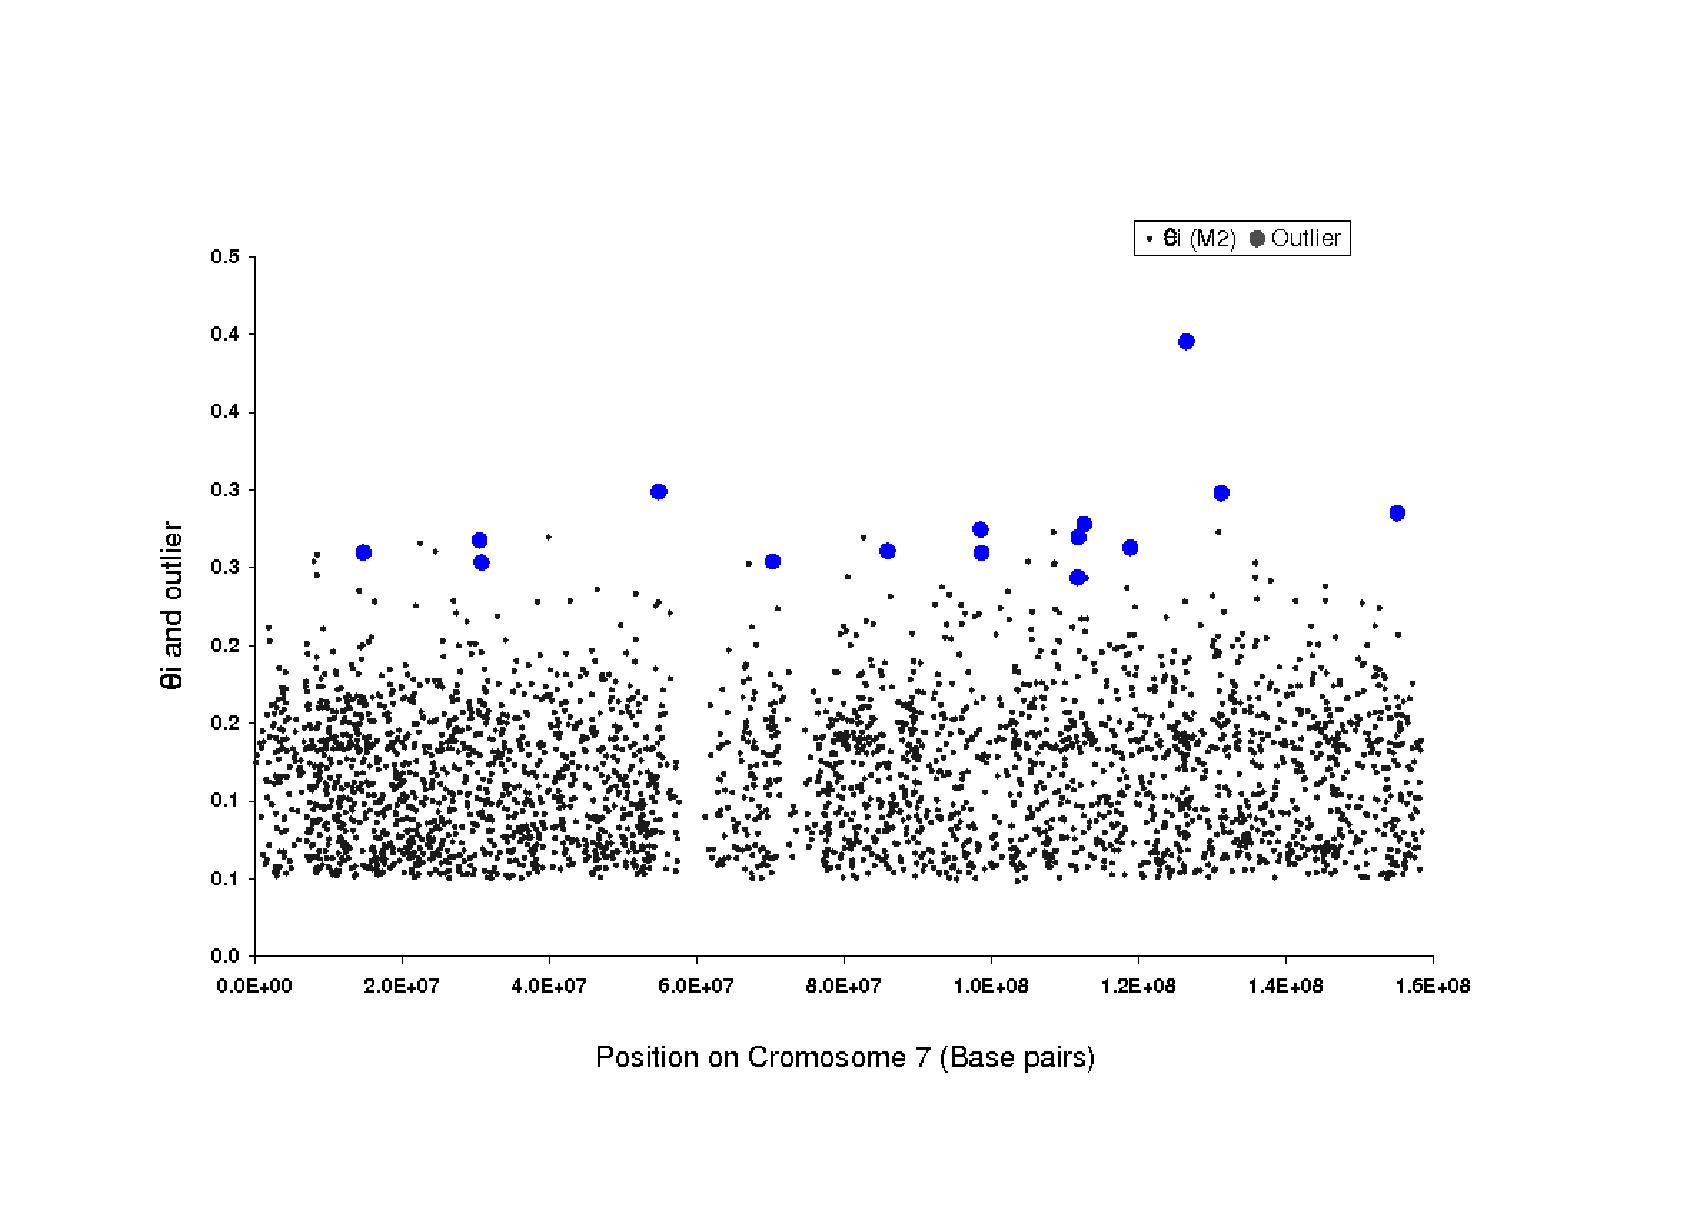
\includegraphics{outlier.eps}}
\end{center}
}

\myslide{
\begin{center}
\resizebox{\textwidth}{!}{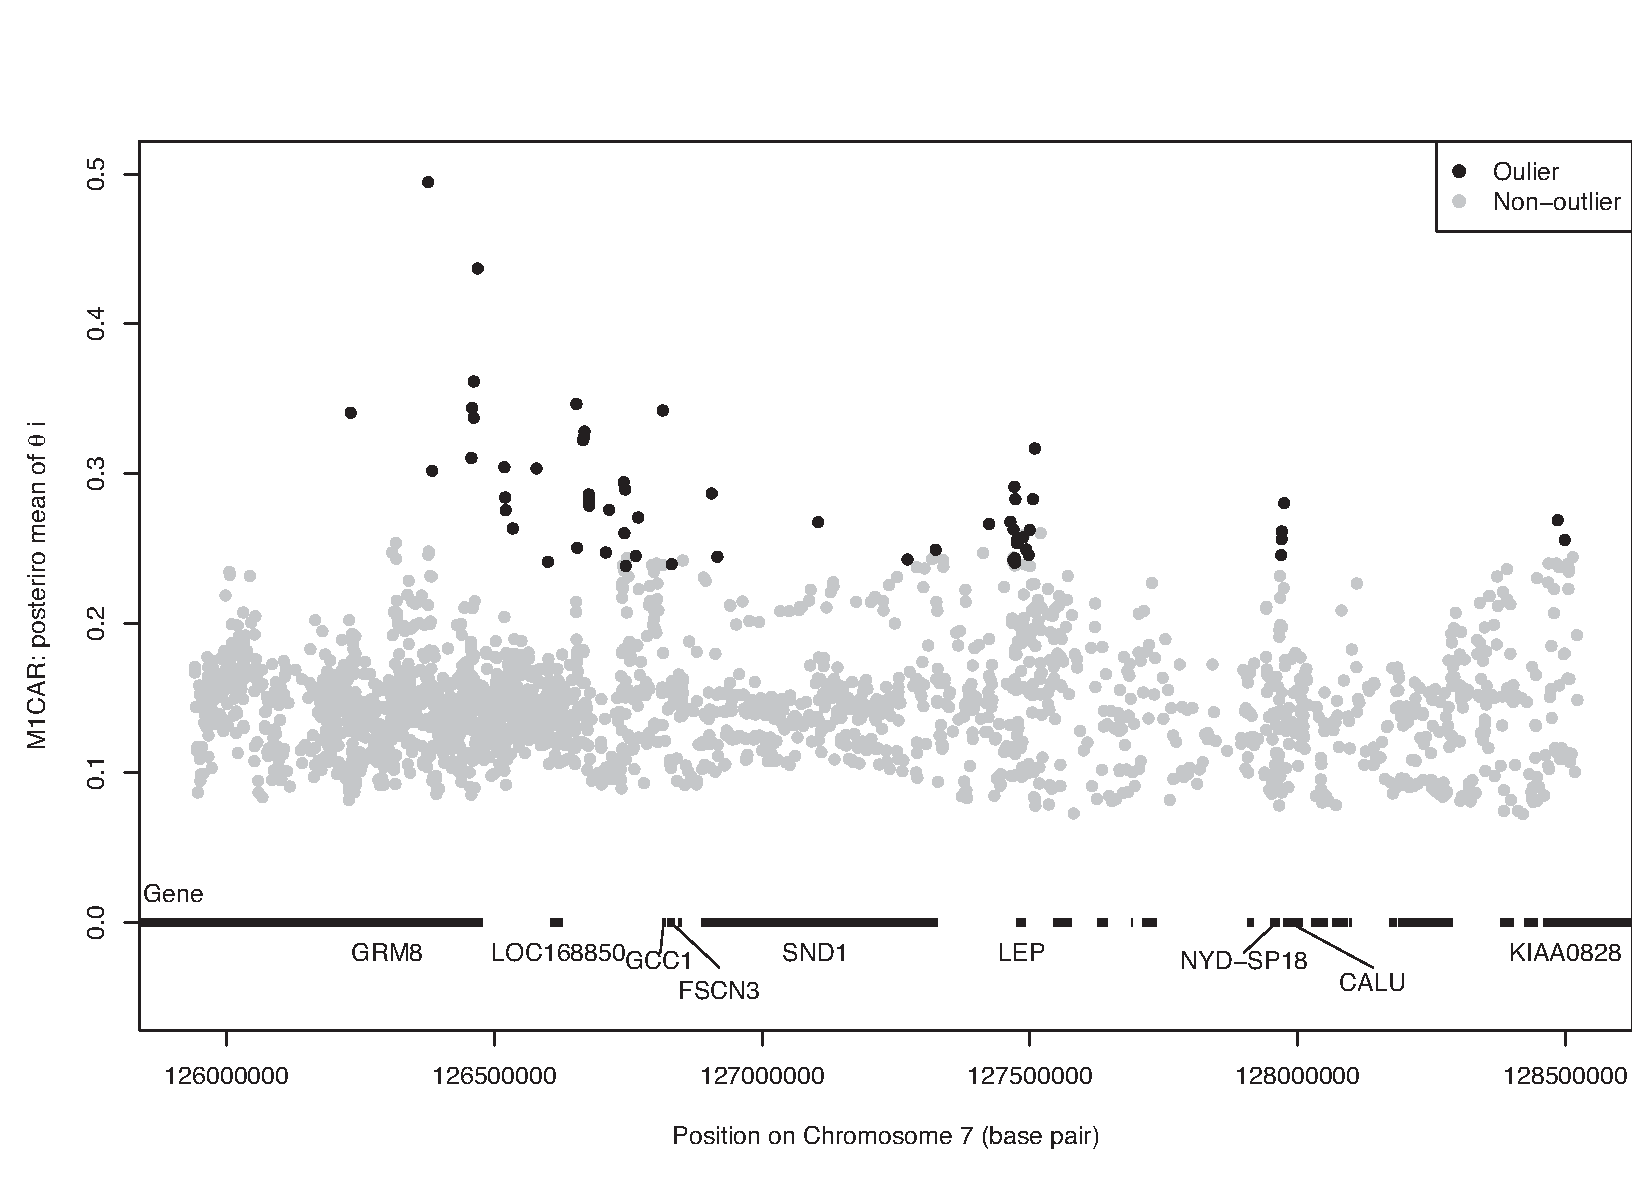
\includegraphics[angle=270]{outlier-high.eps}}
\end{center}
}

\myslide{
\begin{center}
\begin{tabular}{lcccccc}
\hline\hline
      & \multicolumn{2}{c}{ARS} 
      & \multicolumn{2}{c}{$\alpha_1$ and $\alpha_2$}
      & \multicolumn{2}{c}{$\alpha_3$} \\
Locus & $K_s$ & $K_a$ & $K_s$ & $K_a$ & $K_s$ & $K_a$ \\
\hline
Human \\
\quad HLA-A & 3.5 & 13.3*** &  2.5 & 1.6 & 9.5 & 1.6** \\
\quad HLA-B & 7.1 & 18.1**  &  6.9 & 2.4 & 1.5 & 0.5 \\
\quad HLA-C & 3.8 &  8.8    & 10.4 & 4.8 & 2.1 & 1.0 \\
Mean        & 4.7 & 14.1*** &  5.1 & 2.4 & 5.8 & 1.1** \\
\\
Mouse \\
\quad H2-K  & 15.0 & 22.9   &  8.7 & 5.8 & 2.3 & 4.0 \\
\quad H2-L  & 11.4 & 19.5   &  8.8 & 6.8 & 0.0 & 2.5** \\
Mean        & 13.2 & 21.2*  &  8.8 & 6.3 & 1.2 & 3.6** \\
\hline
\end{tabular}
\end{center}
}

\myslide{
\[
\pi = \sum x_ix_j\delta_{ij}/N \quad .
\]
\vfill
\begin{eqnarray*}
\E(\pi) &=& \theta \\
\E(k) &=& \theta\sum_i^{n-1} \frac{1}{i} \quad ,
\end{eqnarray*}
\begin{eqnarray*}
\hat \theta_\pi &=& \hat \pi \\
\hat \theta_k   &=& \frac{k}{\sum_i^{n-1}\frac{1}{i}} \quad ,
\end{eqnarray*}
\vfill
\[
\hat D = \hat\theta_\pi - \hat\theta_k 
\]
}

\myslide{
\begin{eqnarray*}
S &=& \mbox{Probability of fewer alleles given observed diversity} \\
F_S &=& \ln\left(\frac{\hat S}{1 - \hat S}\right)
\end{eqnarray*}
}

\myslide{
\[
\mbox{E}(\xi_i) = \frac{\theta}{i} \quad .
\]
\begin{eqnarray*}
\hat\theta_\pi &=& {n \choose 2}^{-1}\sum_{i=1}^{n-1}i(n-i)\hat\xi_i \\
\hat\theta_k  &=& \frac{1}{a_n}\sum_{i=1}^{n-1}\hat\xi_i \\
&& \\
\theta_H &=& {n \choose 2}^{-1}\sum_{i=1}^{n-1}i^2\hat\xi_i \\
\theta_L &=& \frac{1}{n-1}\sum_{i=1}^{n-1}i\hat\xi_i
\end{eqnarray*}
}

\myslide{
\vfill
\begin{eqnarray*}
\theta_H &=& {n \choose 2}^{-1}\sum_{i=1}^{n-1}i^2\hat\xi_i \\
\theta_L &=& \frac{1}{n-1}\sum_{i=1}^{n-1}i\hat\xi_i \\
&& \\
H &=& \hat\theta_\pi - \theta_H  \\
E &=& \theta_L - \theta_k 
\end{eqnarray*}
}


\end{document}


